\section{Thermodynamik }
\label{sec:Thermodynamik}

In diesem Kapitel wird in Abschnitt \ref{subsec:Kaltdampf-Kaelteprozess} die Thermodynamik des Kaltdampf-Kälteprozess näher beschrieben, um danach die Thermodynamik der feuchten Luft in Abschnitt \ref{subsec:Feuchte Luft} und die Entstehung von Eiskristallen in Abschnitt \ref{subsec:Reifbildung} zu erklären. Zum Schluss des Kapitels werfen wir einen Blick auf die Morphologie von Eiskristallen und ihre physikalischen Eigenschaften.


\subsection{Kaltdampf-Kälteprozess}
\label{subsec:Kaltdampf-Kaelteprozess}



Ein Verdampfer hat die Aufgabe einer Umgebung Energie in Form von Wärme zu entziehen. Hierfür wird in einem Wärmeübetrager flüssiges Kältemittel verdampft. Das verdampfende Kältemittel kühlt zunächst den Wärmeübertrager, danach wird über die Wärmeübertrager-Lamellen der vorbei strömende Luft Wärme entzogen.
Der Kaltdampf-Kälteprozess ist ein linksläufiger \textit{Clausius-Rankine-Kreisprozess}. Die Zustandspunkte des verwendeten Kältemittels im log p,h Diagramm sind in Abbildung \ref{fig:Schema p-h-Diagramm} dargestellt. 

\begin{figure}[htb]
\centering		
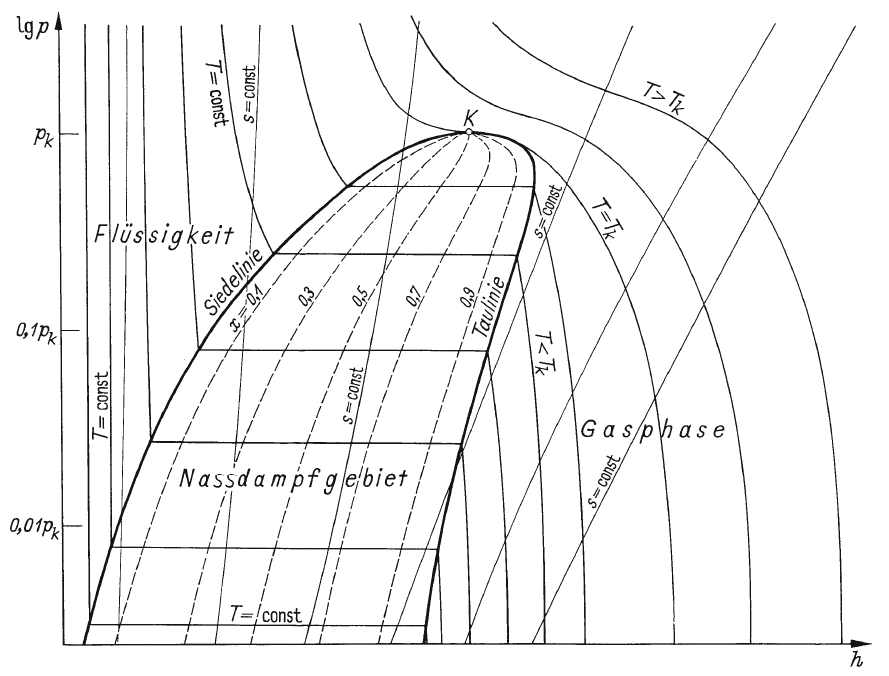
\includegraphics[width=0.75\textwidth]{Pictures/log_p_h_Beahr_Schema.png}
\caption{log p,h-Diagramm von eines reinen Fluids  \citep{Baehr2013}}
\label{fig:Schema p-h-Diagramm}
\end{figure}

Das halb-logarithmische Diagramm ist ein vielgebrauchtes und hilfreiches Mittel in der Kältetechnik. 
\footnote{Das Zustandsdiagramm wurde vom deutschen Ingenieur Richard Mollier (1863-1935) im Jahre 1924 erstmalig vorgestellt.} 
Der Druck logarithmisch auf der y-Achse und die spezifische Enthalpie $h$ auf der x-Achse eingetragen. Die Siedelinie ist durch $x = 0$ und die Taulinie durch $x = 1$. Zwischen $0\leqq x\leqq 1$ befindet sich das Nassdampfgebiet. Es liegt ein Gemisch aus gasförmigen und flüssigem Kältemittel vor. Der Anteil des Gases im Nassdampfgebiet wird durch $x$ ausgedrückt; $1-x$ ist der Anteil der Flüssigkeit.


In dem Diagramm \ref{fig:Komponeneten und p-h-Diagramm} sind alle Zustandspunkte bei einem Durchlauf des Kältekreislaufes abgebildet. Innerhalb des Nassdampfgebietes verläuft in einem idealen Kältekreislauf, eine Zustandsänderung \textit{isotherm} und \textit{isobar} ab. Wärmezu- oder abfuhr führt nicht zu einer Erhöhung der Temperatur, sondern zu einer Veränderung vom Gas- bzw. Flüssigkeitsanteil. Es wird von einer \textit{latenten}, also nicht fühlbaren,  Wärmeänderung gesprochen. Um einen Tropfen flüssigen Wasser, dessen Zustand sich auf der Siedelinie befindet, in einen gasförmigen Zustand, sprich $x=1$ zu überführen, muss ihm die spezifische Verdampfungsenthalpie $\Delta h$ zugeführt werden. Verläuft die Zustandsänderung entgegengesetzt, kondensiert der Tropfen und gibt die Verdampfungsenthalpie $\Delta h$ an seine Umgebung ab. 
Außerhalb des Nassdampfgebietes führt eine Wärmezu- oder abfuhr zu einer Veränderung der Temperatur. Die Wärmeänderung ist \textit{sensibel}. 

\begin{figure}[htb]
\centering		
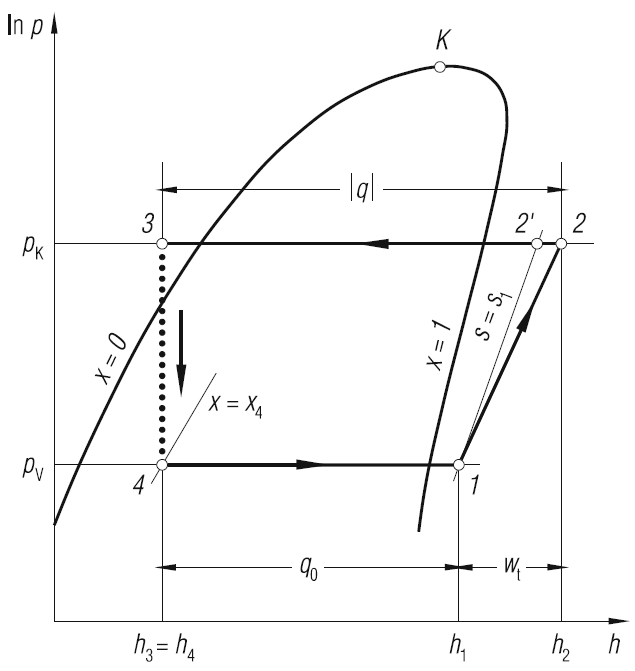
\includegraphics[width=0.6\textwidth]{Pictures/log_p_h_Beahr.png}
\caption{Kreisprozess im log p,h-Diagramm \citep{Baehr2013}}
\label{fig:Komponeneten und p-h-Diagramm}
\end{figure}


In einem  Kaltdampfprozess, sprich ohne Verluste durch Reibung (\textit{reversibel}), finden folgende vier Teilprozesse statt:

\begin{itemize}
\item[1 $\longrightarrow$ 2] Kompression des dampfförmigen Kältemittels unter der Zuführung von elektrischer Leistung $P_{KM}$
\item[2 $\longrightarrow$ 3] Abkühlung, Kondensation und Unterkühlung des Kältemittels unter der Abgabe der Wärmeenergie $\dot{Q}$ über den Verflüssiger an die Umgebung
\item[3 $\longrightarrow$ 4] Entspannung des flüssigen Kältemittels durch das Drosselventil; teilweise setzt die Verdampfung des Fluids ein 
\item[4 $\longrightarrow$ 1] Verdampfung des noch flüssigen Kältemittels auf niedrigem Druckniveau unter der Aufnahme des Wärmestromes $\dot{Q_0}$ aus dem Kühlraum
\end{itemize}

Der Prozess findet auf zwei Druckniveaus statt: dem Verdampfungsdruck $p_V$ und dem Kondensationsdruck $p_K$. Die Verflüssigung des Kältemittels findet auf hohem Druckniveau und die Verdampfung auf niedrigem Druck statt. Die höchste Temperatur wird nach der Kompression am Zustandspunkt 2 erreicht; er befindet sich im Überhitzen- und Hochdruckbereich. Die niedrigste Temperatur ist kurz nach dem Dosselventil und vor dem Verdampfer am Punkt 4. auf niedrigem Druckniveau. 

Nach dem Anwenden des 1. Hauptsatzes der Thermodynamik, die Erhaltung der Energie in einem System, auf den Kältekreislauf folgt die Gleichung :

 \begin{equation}
 	|\dot{Q}|  = \dot{Q_0} +  P_{KM}.
 	\label{eq:Energiebilanz}
 \end{equation}
 
Die elektrische Antriebsleistung der Kältemaschine ist die aufgenommene elektrische Leistung durch den Kompressor zwischen den Zustandspunkten 1  und 2. Sie ergibt sich zu:

\begin{equation}
P_{KM} = \dot{m}~ w_t= \dot{m}~ (h_2 - h_1) = \frac{\dot{m} }{\eta_{sV}} (h_{2'}- h_1).
\label{eq:Antriebsleistung}
\end{equation}

Hierbei ist $\eta_{sV}$ der isentrope Wirkungsgrad des Kompressors. Der isentrope Wirkungsgrad setzt den realen Kältekreislauf in ein Verhältnis zum idealen Kältekreislauf. Die Überhitzung des Gases am Austritt des Kompressors ist höher als die Überhitzung nach einer isentropen Verdichtung. Daraus folgt eine höhere Energieaufnahme durch den Kompressor und ein höherer Wärmestrom $\dot{Q}$, der über den Verflüssiger an die Umgebung abgegeben werden muss. Der isentrope Wirkungsgrad ist definiert über 

\begin{equation}
\eta_{sV}:= \frac{h_{2'}- h_{1}}{h_2 - h_1}.
\label{eq:Antriebsleistung}
\end{equation}


Der Wärmestrom $\dot{Q}$ wird über den Verflüssiger zwischen den Zuständen 2 und 3 abgeführt. Die Formel von  $\dot{Q}$ lautet: 

\begin{equation}
	\dot{Q} = \dot{m}~q_0 = \dot{m}~ (h_3 - h_2)< 0.
	\label{eq:Wärmestrom}
\end{equation}

Der Wärmestrom $\dot{Q}$ ist immer kleiner als Null; er wird dem Kreislauf folglich entzogen.  
 
Über ein Drosselorgan wird das Kältemittel vom hohen Druckniveau auf das niedrigere Druckniveau entspannt. Der Teilprozess findet zwischen den Zustandspunkten 3 und 4 statt und wird als $isenthalp$ angenommen.  
 
Die Kälteleistung $\dot{Q_0}$, sprich der aus dem Kühlraum zu entnehmender Wärmestrom, ergibt sich aus dem Kältemittel-Massenstrom $\dot{m}$ und den spezifischen Enthalpien der Zustände 4 und 1 :

\begin{equation}
	\dot{Q_0} = \dot{m}~ q_0 = \dot{m}~ (h_1 - h_4).
	\label{eq:Kälteleistung}
\end{equation}




Die Bewertung einer Kälteanlage erfolgt durch die Leistungszahl $\epsilon_{KM}$: 

\begin{equation}
	\epsilon_{KM} := \frac{Kälteleistung}{Antriebsleistung} =\frac{\dot{Q_0}}{P_{KM}}.
	\label{eq:Leistungszahl}
\end{equation}

Ziel bei der Auslegung und dem Betrieb einer Kältemaschine ist es eine möglichst große Leistungszahl zu erlangen.

\subsection{Feuchte Luft}
\label{subsec:Feuchte Luft}

Bei dem Kühlprozess durch einen Verdampfer kommt es zwischen dem Wärmeübertrager und der feuchten Luft zu verschiedenen thermodynamischen Phänomenen. Die auftretenden Phänomene lassen sich in folgende Gruppen einordnen:

\begin{itemize}
\item	Abkühlung der feuchten Luft 
\item 	Wassertropfenbildung auf Lamellenoberfläche
\item	Kristallbildung auf Lamellenoberfläche. (siehe Abschnitt \ref{subsec:Reifbildung})
\end{itemize}

In diesem Abschnitt  wird zunächst die Thermodynamik der feuchten Luft thematisiert. 


\begin{figure}[htb]
\centering		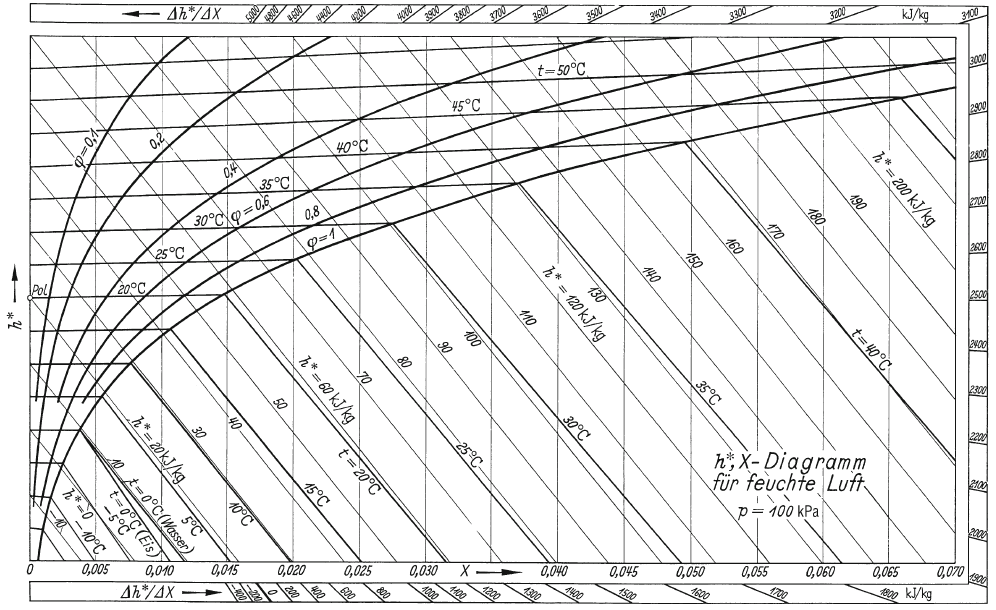
\includegraphics[width=0.85\textwidth]{Pictures/h_x_Diagramm_Beahr.png}
\caption{$h^*$, $X$- Diagramm für feuchte Luft bei einem Gesamtdruck $p= $ 100 kPa \citep{Baehr2013}}
\label{fig:h_x_diagramm}
\end{figure}


Bei dem Wärmeentzug durch den Verdampfer wird  zunächst die noch nicht gesättigte feuchte Luft abgekühlt. Luft besitzt die Eigenschaft eine bestimmte Menge Wasser aufnehmen zu können. Warme Luft kann mehr Wasser aufnehmen als kalte Luft. Das Verhältnis von der aufgenommene Masse Wasser zur Masse Luft ist definiert als Beladung: 

\begin{equation}
X = \frac{m_W}{m_L}.
\label{eq:Beladung}
\end{equation}

In dieser Formel bezieht sich $m_W$ auf gasförmige, flüssige oder feste Form von Wasser und $m_L$ auf die Masse der trockenen Luft.  $X$ kann Werte zwischen 0 für trockene Luft und $\infty$ für reines Wasser annehmen. In der Regel bleibt $X$ jedoch kleiner als 0,1. 

Die absolute Feuchte ist definiert als das Verhältnis von Masse des Wasserdampfers $m_W$ zum eingenommen Volumen $V$ der feuchten Luft. Die Formel lautet: 

\begin{equation}
\varrho := \frac{m_W}{V} = \frac{p_w}{R_W T}.
\label{eq:Absolute Feuchte}
\end{equation}


Die relative Feuchte $\varphi$ ist das Verhältnis der absoluten Feuchte im Verhältnis zum Maximalwert oder Sättigungswert der absoluten Feuchte: 

\begin{equation}
 \varphi := \frac{\varrho}{\varrho_W^s}.
 \label{eq:Rel Feuchte}
\end{equation}

Wird nun in die Gleichung \ref{eq:Beladung} die relative Feuchte aus Gleichung \ref{eq:Rel Feuchte} eingesetzt, ergibt sich eine weitere Formel für die Beladung $X$. 

\begin{equation}
X = \frac{m_W}{m_L} = 0,622 \frac{p_{W}^s}{p/\varphi - p_{W}^s}.
\label{eq:Beladung 2}
\end{equation}

Hierbei ist $p_{W}^s$ der Partialdruck des Sättigungspunktes.
Betrachtet man nur die Wasserdampfbeladung der Luft, so lässt sich feststellen, dass die maximale Menge an aufzunehmendem Wasser einen Grenzwert hat. Dieser Grenzwert wird Sättigungswert der Wasserdampfbeladung genannt und ist eine Funktion, die abhängig von der Temperatur und dem Druck ist.  Sie berechnet sich nach dem Gesetz von Dalton zu :

\begin{equation}
 X_s (T,p) = 0,622 \frac{p_{W}^s}{p - p_{W}^s}.
 \label{eq:Sättigungsbeladung}
\end{equation}

Bei der Abkühlung von feuchter Luft kann der Fall eintreten, dass $X > X_s$ ist. Sprich, die Beladung der trockenen Luft ist größer als die Menge an Wasser, die im Wasserdampf aufgenommen werden kann. Der erste Tropfen Kondensat bildet sich und Wasser fällt aus. Wird das ausgefallene Wasser mit der Luft weitertransportiert, so wird von \textit{Nebel} geredet. Die Kondensationsmenge lautet formelmäßig:

\begin{equation}
\Delta X m_L = (X - X_s)m_L.
\label{eq:Delta_X}
\end{equation}

Die Wassermenge $X_s m_L$ ist gasförmig von der trockenen Luft gespeichert. Die Kondensationsmenge $\Delta X m_L$ setzt sich nun an Keimpunkten in der Umgebung ab oder wird als Nebel aus der Gasphase ausgeschieden. Keimzellen für Wassertropfen können zum Beispiel Verunreinigungen oder raue Oberflächen sein. Das höchste treibende Potential für eine solche Keimzelle hat der kälteste Punkt im System. In unserem Anwendungsfall ist das der Wärmeübertrager des Verdampfers. Da der Verdampfer zur Bereitstellung der Kälteleistung und einer funktionierenden Wärmeübertragung stets eine Temperaturdifferenz zwischen dem Kältemittel und der vorbei strömenden Luft  bereitstellt,  bilden sich hier die ersten Tropfen. Je nach ursprünglicher Beladung der Luft bilden sich die Tropfen eher am Anfang oder Ende des Wärmeübertragers. War die feuchte Luft schon vor dem Eintritt in den Wärmeübertrager bereits stark gesättigt, bilden sich Tropfen am Eingang der Lamellen. \citep{Danfoss2006}

Die feuchte Luft überträgt beim Durchströmen des Luftkühlers durch die Kondensation auf der Lamellenoberfläche Wärme an die selbige. Der übertragene Wärmestrom ist, ausgehend von der Luft, formelmäßig gegeben mit: 

\begin{equation}
\dot{Q}= \dot{m}_L (c_{pL}\Delta T + h_v \Delta X)
\label{eq:Wärmestrom feuchte luft}
\end{equation}

%An der Formel \ref{eq:Wärmestrom feuchte luft} lässt sich erkennen, dass die Kondensation von Wasser auf dem Wärmeübertrager zunächst einen positiven Effekt auf die Luftkühlung hat.
 Es wird mehr Wärme von der Luft auf das Kältemittel übertragen. Bei der Kondensation wird neben der sensiblen Wärme zusätzlich latente Wärme abgegeben. Der latente Teil der Wärme, die Verdampfungsenthalpie $h_v$, ist durch den zweiten Term in der Formel gegeben. 

Gefriert das Kondensat zusätzlich, erhöht sich der Term der latenten Wärme um die Schmelzenthalpie $h_s$. Die Formel für den übertragenden Wärmestrom lautet in diesem Falle: 

\begin{equation}
\dot{Q}= \dot{m}_L (c_{pL}\Delta T + (h_v+ h_s) \Delta X)
\label{eq:Wärmestrom Reif}
\end{equation}

\citep{Grote2014}
\citep{Baehr2013}

\subsection{Reif- und Eisbildung}
\label{subsec:Reifbildung}

Liegt die Oberflächentemperatur auf dem Wärmeübertrager des Verdampfers nicht nur unter dem Taupunktpunkt der feuchten Luft, sondern auch unter dem Gefrierpunkt, kann es zum Gefrieren der kondensierten Tropfen und/oder zur Desublimation von Wasserpartikeln auf der Oberfläche kommen. Dieser Abschnitt soll einen Überblick über diese zwei thermodynamischen Phänome geben. Da in dieser Arbeit nicht der Reifbildungsprozess im Hauptfokus steht, sondern  der technische Aspekt der Abtauung, wird der Eisbildungsprozess hier nur kurz erläutert.

In der Literatur gibt es zahlreiche Quellen, die sich mit der Reif- bzw. Eisbildung auseinander setzen. Die Quellen beschreiben den Kristallbildungsprozess sowohl aus der rein theoretischer Sicht als auch mittels simulationsrelevanten und technischen Überlegungen bzw. Untersuchungen. Der scheinbar triviale Prozess der Bildung eines Eiskristalles auf einer Oberfläche und sein weiteres Wachstumsverhalten ist sehr komplex und Gegenstand zahlreicher aktueller und schon abgeschlossener Forschungsprojekte.

Neben den theoretischen Grundlagen wird in der Arbeit von \textsc{\citeauthor{Schydlo2010}} ein Simulationsmodell für den Reifbildungs- und Abtauprozess auf einem Rohr entwickelt. Zudem sind bisherige Arbeiten zu der Thematik in \citep{Schydlo2010} aufgelistet und zusammengefasst. 
Praktische Untersuchungen sowie Versuchsaufbauten zum Thema der Vereisung von Luftkühlern werden in \textsc{\citeauthor{Sahinagic2004}} und \textsc{\citeauthor{Kosowski2009}} beschrieben. In den Arbeiten werden die Vereisungs- und innovative Abtauungsprozesse von einer CO$_2$-Wärmepumpe, die zur Heizung von Passivhäuser eingesetzt wird, untersucht.   



Es gibt zahlreiche Einflussgrößen, die auf den Prozess und die Form des Eiskristalls und späteren Reif einwirkten. 
  Die wichtigsten Einflussgrößen sind die Luftgeschwindigkeit, die Lufttemperatur, die Luftfeuchte, die Oberflächentemperatur und die Zeit. Um den Reif charakterisieren zu können, werden folgende Größen zur Hilfe genommen: die Reifdicke, die Reifdichte, die Porösität und die Wärmeleitfähigkeit. 

In der Arbeit von \textsc{\citeauthor{Hayashi1977}} aus dem Jahre 1977 wird der Eiskristallwachstum in drei Phasen unterteilt:

\begin{enumerate}
\item Eindimensionales Kristallwachstum
\item Reifschichtwachstumsphase 
\item Vergletscherung.
\end{enumerate}


\begin{figure}[htb]
\centering		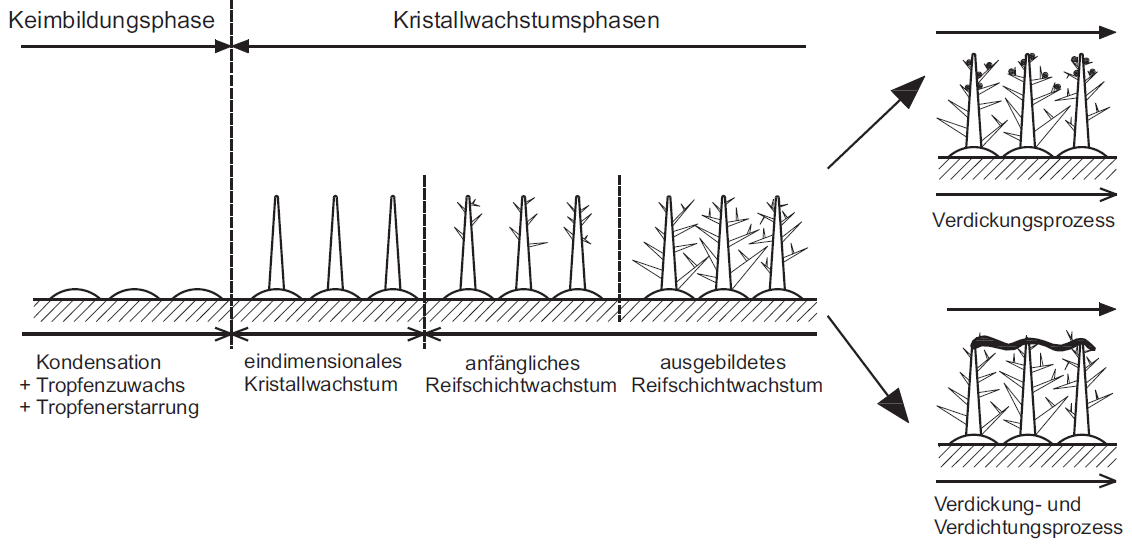
\includegraphics[width=0.85\textwidth]{Pictures/Reifbildungsphasen_Schydlo.png}
\caption{Kristallwachstum auf einer ebenen Oberfläche \citep{Schydlo2010}}
\label{fig:Kristallwachstum}
\end{figure}


In Abbildung \ref{fig:Kristallwachstum} sind die drei Kristallwachstums-Phasen nach \textsc{\citeauthor{Hayashi1977}} sowie die vorhergehende Keimbildungsphase, eingeführt in \citep{Sahinagic2004}, dargestellt. 

\subsubsection*{Keimbildungsphase}

In der Keimbildungsphase bilden sich zunächst Wassertropfen auf der Lamellenoberfläche, die trotz Temperaturen kleiner als der Gefrierpunkt nicht erstarren, sondern zu größeren Tropfen anwachsen. Je kleiner die Unterkühlung, desto größer werden die Tropfen, bevor sie erstarren und in die erste Kristallwachstumsphase übergehen. 

\subsubsection*{Eindimensionales Kristallwachstum}
Die erste Phase ist gekennzeichnet durch Kristallwachstum senkrecht zur Oberfläche und mit einheitlicher Wachstumsgeschwindigkeit. Dies führt aufgrund der sich stetig vermehrenden Kristalle zu einer erhöhten Rauigkeit.  

\subsubsection*{Reifschichtwachstumsphase}
In der zweiten Phase beginnt das dreidimensionale Wachstum. Die Kristalle fangen an sich miteinander zu verästeln. Ein poröses Kristallgitter entsteht. Aufgrund des  Wärmeleitwiderstandes, der mit der Reifdicke steigt, erhöht sich die Oberflächentemperatur der Reifschicht. Des weiteren kommt es zu einem Massenstrom innerhalb der Reifschicht, ausgelöst durch Diffusion. Die Diffusion rührt aus  dem  Konzentrationsunterschieden zwischen der Lamelle und der Reifoberfläche. Der Wassermassenstrom läuft in das poröse Kristallgitter und gefriert dort in Nähe der Lamelle. Die Dichte der Reifschicht steigt und mit ihr der Wärmewiderstand. Dies führt zu einer Erhöhung der Oberflächentemperatur der Reifschicht und schließlich zur Überschreitung des Gefrierpunktes von Eis. Die Spitzen des Kristalle schmelzen und es bildet sich Kondensat. Die dritte Wachstumsphase beginnt. 

\subsubsection*{Vergletscherung}

Das flüssige Wasser läuft aufgrund der Kapillarwirkung der Kristalle in die Zwischenräume des Kristallgitters und gefriert dort wieder. Die Kristallgitter werden dichter und kompakter. Dies führt zur Steigerung der Wärmeleitfähigkeit der Reifschicht. Es wird von einer Vergletscherung gesprochen. Die Oberflächentemperatur der Reifschicht sinkt erneut und fällt erneut unter den Gefrierpunkt. Nun kann die feuchte Luft erneut an der Oberfläche des Reifs desublimieren. Der Prozess wiederholt sich solange, bis das Eis so kompakt ist, dass kein weiteres Kondensat mehr in die Reifschicht eindringen kann. 

\subsection*{Physikalische Eigenschaften von Eiskristallen}

 Im vorangegangenen Abschnitt \ref{subsec:Reifbildung} wurden die einzelnen Bildungsphasen von Eiskristallen beschrieben. In diesem Abschnitt wird auf die Eigenschaften von Eiskristallen eingegangen und dargestellt wie sie sich während eines Vereisungsvorganges eines Luftkühlers verändern. 
 
Gefriert ein Tropfen Wasser und wird zum Eiskristall, so verändern sich die physikalischen Eigenschaften des Tropfens. In der Arbeit von \textsc{\citeauthor{Schydlo2010}} verdeutlichen zunächst zwei Diagramme, abgebildet in \ref{fig:Zeitverlaufe von Reifdichte und -dicke}, wie sich die Reifdicke und die Reifdichte während eines Vereisungsvorgang verändern. 

\begin{figure}
\centering
    \subfigure[Reifdichte]
    {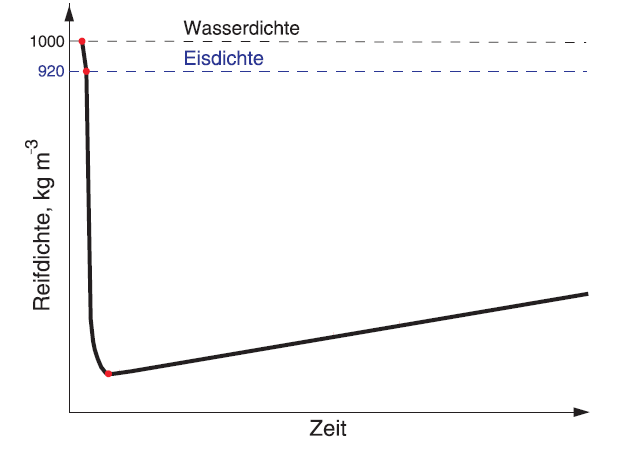
\includegraphics[width=0.50\textwidth]{Pictures/Reifdichte_Schydlo.png}}
    \subfigure[Reifdicke]{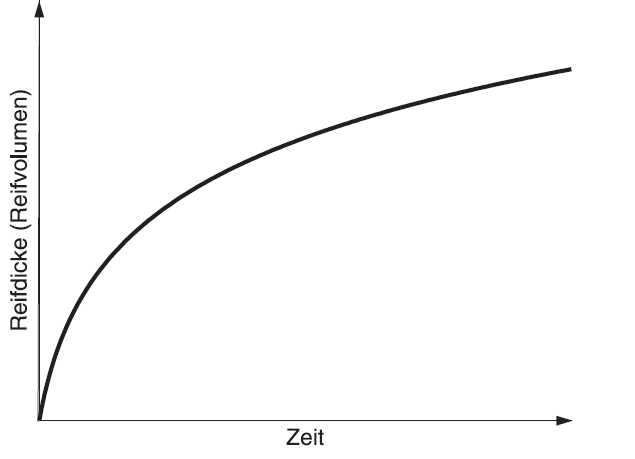
\includegraphics[width=0.48\textwidth]{Pictures/Reifdicke_Schydlo.png}}
\caption{Schematischer Reifdichte- und Reifdickeverläufe beim Vereisungsvorgang eines Tropfen Wassers \citep{Schydlo2010}}
\label{fig:Zeitverlaufe von Reifdichte und -dicke}
\end{figure}

Da Diagramm \ref{fig:Zeitverlaufe von Reifdichte und -dicke}(a) zeigt den Dichteverlauf, aufgetragen über die Vereisungszeit. Die Dichte eines Tropfens fällt beim Gefrieren von 1000 kg/m$^3$ auf 920 kg/m$^3$ sinkt. Danach tritt das in Abschnitt \ref{subsec:Reifbildung} beschriebene eindimensionale Wachstum ein, sodass die Reifdichte bis auf ein Minimum fällt. Danach tritt die dreidimensionale Wachstumsphase und dann die Vergletscherungsphase ein. Die Dichte  steigt jetzt langsam, aber kontinuierlich wieder an.

\begin{figure}[htb]
\centering	
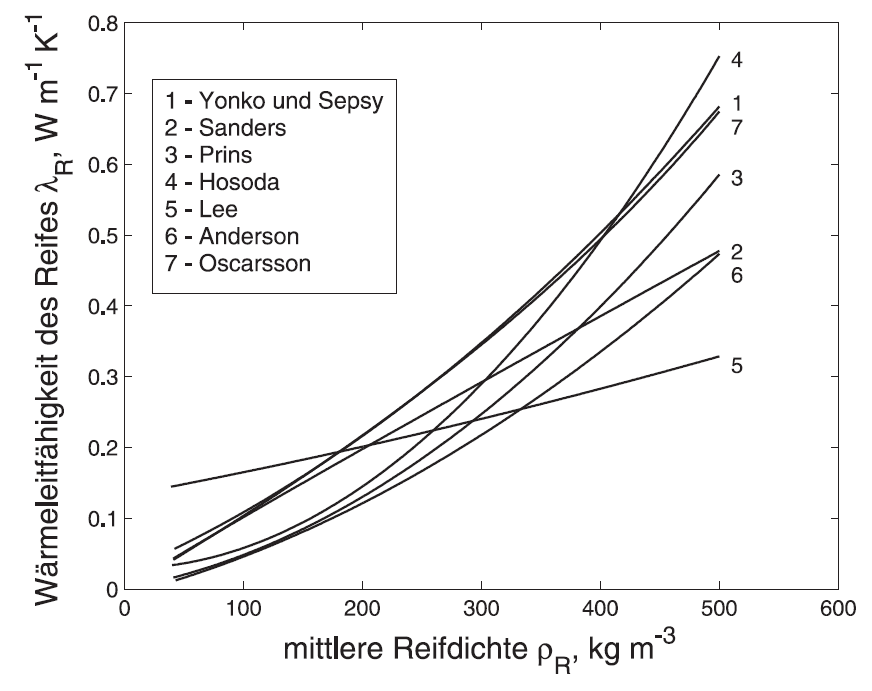
\includegraphics[width=0.55\textwidth]{Pictures/Waermeleitfaehigkeit_Schydlo.png}
\caption{Wärmeleitfähigkeit des Reifs aufgetragen über die mittlere Reifdichte \citep{Schydlo2010}}
\label{fig:Waermeleitfaehigkeit}
\end{figure}

Im \ref{fig:Zeitverlaufe von Reifdichte und -dicke}(b) ist der Reifdickenverlauf aufgetragen. Aus diesem lässt sich entnehmen, dass kurz nach Beginn die zeitliche Änderung der Reifdicke maximal ist. Das heißt, dass der Massenstrom an Kondensat, das sich an der Lamelle absondert und dann gefriert, am Anfang am größten ist und findet während des eindimensionalen Wachstums auf statt. Beim dreidimensionalen Wachstum und späteren Vergletscherung flacht die Kurve ab und strebt gegen einen Sättigungswert. 


 
Mit der Reifdicke verändert sich wiederum die Wärmeleitfähigkeit des Reifes, abgebildet in \ref{fig:Waermeleitfaehigkeit}. In dem Diagramm sind mehrere Berechnungsmodelle aufgetragen, die die Wärmeleitfähigkeit als Funktion der mittleren Reifdichte abbilden. Alle Modelle sagen einen Anstieg von $\lambda$ mit steigender Reifdichte voraus. Dies hängt mit der Verdichtung des Eises während der Vergletscherungsphase zusammen. Die führt dazu, dass Reif mit einer geringen Dichte gleichzeitig als sehr guter Isolator fungiert. \citep{Baehr2013}  \citep{Kosowski2009}


